\documentclass[11pt]{article}
\usepackage{tabularx}

% Change "review" to "final" to generate the final (sometimes called camera-ready) version.
% Change to "preprint" to generate a non-anonymous version with page numbers.
\usepackage[review]{acl}

% Standard package includes
\usepackage{times}
\usepackage{latexsym}
\usepackage{amsmath}
\usepackage{comment}
\usepackage{booktabs}
\usepackage{longtable}
\usepackage{subcaption}

% For proper rendering and hyphenation of words containing Latin characters (including in bib files)
\usepackage[T1]{fontenc}
% For Vietnamese characters
% \usepackage[T5]{fontenc}
% See https://www.latex-project.org/help/documentation/encguide.pdf for other character sets

% This assumes your files are encoded as UTF8
\usepackage[utf8]{inputenc}

% This is not strictly necessary, and may be commented out,
% but it will improve the layout of the manuscript,
% and will typically save some space.
\usepackage{microtype}

% This is also not strictly necessary, and may be commented out.
% However, it will improve the aesthetics of text in
% the typewriter font.
\usepackage{inconsolata}

%Including images in your LaTeX document requires adding
%additional package(s)
\usepackage{graphicx}

% If the title and author information does not fit in the area allocated, uncomment the following
%
%\setlength\titlebox{<dim>}
%
% and set <dim> to something 5cm or larger.

\title{Search+: Structuring Retrieved Context with Query-Aware Textual Graphs for Multi-Hop Retrieval}

% Author information can be set in various styles:
% For several authors from the same institution:
% \author{Author 1 \and ... \and Author n \\
%         Address line \\ ... \\ Address line}
% if the names do not fit well on one line use
%         Author 1 \\ {\bf Author 2} \\ ... \\ {\bf Author n} \\
% For authors from different institutions:
% \author{Author 1 \\ Address line \\  ... \\ Address line
%         \And  ... \And
%         Author n \\ Address line \\ ... \\ Address line}
% To start a separate ``row'' of authors use \AND, as in
% \author{Author 1 \\ Address line \\  ... \\ Address line
%         \AND
%         Author 2 \\ Address line \\ ... \\ Address line \And
%         Author 3 \\ Address line \\ ... \\ Address line}

\author{First Author \\
  Affiliation / Address line 1 \\
  Affiliation / Address line 2 \\
  Affiliation / Address line 3 \\
  \texttt{email@domain} \\\And
  Second Author \\
  Affiliation / Address line 1 \\
  Affiliation / Address line 2 \\
  Affiliation / Address line 3 \\
  \texttt{email@domain} \\}

%\author{
%  \textbf{First Author\textsuperscript{1}},
%  \textbf{Second Author\textsuperscript{1,2}},
%  \textbf{Third T. Author\textsuperscript{1}},
%  \textbf{Fourth Author\textsuperscript{1}},
%\\
%  \textbf{Fifth Author\textsuperscript{1,2}},
%  \textbf{Sixth Author\textsuperscript{1}},
%  \textbf{Seventh Author\textsuperscript{1}},
%  \textbf{Eighth Author \textsuperscript{1,2,3,4}},
%\\
%  \textbf{Ninth Author\textsuperscript{1}},
%  \textbf{Tenth Author\textsuperscript{1}},
%  \textbf{Eleventh E. Author\textsuperscript{1,2,3,4,5}},
%  \textbf{Twelfth Author\textsuperscript{1}},
%\\
%  \textbf{Thirteenth Author\textsuperscript{3}},
%  \textbf{Fourteenth F. Author\textsuperscript{2,4}},
%  \textbf{Fifteenth Author\textsuperscript{1}},
%  \textbf{Sixteenth Author\textsuperscript{1}},
%\\
%  \textbf{Seventeenth S. Author\textsuperscript{4,5}},
%  \textbf{Eighteenth Author\textsuperscript{3,4}},
%  \textbf{Nineteenth N. Author\textsuperscript{2,5}},
%  \textbf{Twentieth Author\textsuperscript{1}}
%\\
%\\
%  \textsuperscript{1}Affiliation 1,
%  \textsuperscript{2}Affiliation 2,
%  \textsuperscript{3}Affiliation 3,
%  \textsuperscript{4}Affiliation 4,
%  \textsuperscript{5}Affiliation 5
%\\
%  \small{
%    \textbf{Correspondence:} \href{mailto:email@domain}{email@domain}
%  }
%}

\begin{document}

\maketitle

\begin{abstract}
Dense retrievers often struggle with complex multi-hop reasoning because they evaluate documents in isolation, missing vital cross-document dependencies. To address this limitation, we introduce Search+, a method that dynamically organizes retrieved documents into a query-aware graph.
\end{abstract}



\section{Introduction}

Information Retrieval (IR) is a key component of modern NLP systems, aimed at selecting relevant documents for a given query. Early approaches relied on lexical matching methods such as term frequency and keyword overlap~\cite{DBLP:journals/ftir/RobertsonZ09}, while recent methods use dense embeddings to capture semantic similarity beyond surface-level matching~\cite{DBLP:journals/tois/ZhaoLRW24}.

However, multi-hop retrieval remains challenging because relevant evidence is often distributed across multiple passages and must be connected through intermediate reasoning steps~\cite{DBLP:conf/iclr/XiongLIDLWMY0KO21}. Most existing systems rank documents independently, ignoring dependencies between passages. This limits their ability to capture structural relationships, causing individually weak but collectively important passages to be overlooked.


Recent research has explored the integration of structured representations such as Knowledge Graphs (KGs), where entities and relations are explicitly represented as relational triples. These approaches have shown promise for multi-hop reasoning by modeling explicit connections between pieces of information~\cite{DBLP:journals/apin/LindersT25, DBLP:journals/computers/OsipjanKKGG25}. Several graph-based retrieval approaches rely on external knowledge graphs, graph neural networks, or graph-aware retrievers~\cite{DBLP:conf/acl/MavromatisK25, DBLP:conf/aaai/0160LRSZD24}. Such approaches increase architectural complexity and frequently reduce interpretability.

In this work, we take a different perspective. Rather than modifying the retriever itself or injecting structured knowledge into embedding representations, we formulate multi-hop retrieval as a problem of \emph{query-aware structural organization}. Specifically, we dynamically organize retrieved passages into a lightweight \emph{textual graph} conditioned on the information need expressed by the query. This was done with the objective of filtering unrelated relations that would introduce noise into the pipeline. In this graph, nodes correspond to retrieved passages, while edges capture contextual relationships derived from shared entities and local knowledge obtained from the query.

The resulting graph acts as an explicit relational organization layer over the retrieval space. We investigate two complementary graph-based ranking strategies. First, we apply a Breadth-First Search (BFS) traversal strategy that prioritizes passages according to their structural proximity to highly relevant contextual regions. Second, we introduce a neighbourhood propagation mechanism that refines retrieval scores through iterative relational evidence aggregation across neighbouring nodes. The proposed framework is called Search+.




%Unlike prior graph-enhanced retrieval methods, our approach does not require external knowledge graphs, graph neural network training, or retriever-specific architectural modifications. Instead, it operates as a lightweight and interpretable post-retrieval framework that can be applied on top of existing sparse and dense retrieval systems.

We evaluate the proposed framework on three multi-hop QA benchmarks: HotpotQA~\cite{yang-etal-2018-hotpotqa}, 2WikiMultiHopQA~\cite{ho-etal-2020-constructing}, and MuSiQue~\cite{trivedi-etal-2022-musique}. Experimental results across both sparse and dense retrievers show consistent improvements in Recall@K and Full Recall@K metrics, suggesting that explicitly organizing retrieved evidence through query-aware relational structure improves multi-hop retrieval effectiveness.

So in this work we propose a \textbf{lightweight, query-aware textual graph framework} that organizes retrieved passages using entity overlap and local relational evidence. Based on this graph, we introduce \textbf{two reranking strategies} leveraging structural traversal and neighborhood-based evidence propagation. We demonstrate \textbf{consistent improvements across both sparse and dense retrievers} on three multi-hop QA benchmarks. Overall, we show that explicitly modeling relational structure improves multi-hop evidence retrieval while preserving an \textbf{interpretable and retriever-agnostic design}. All the data, code, and produced graphs are available at the link~\footnote{\url{https://anonymous.4open.science/r/Search--61D8/README.md}}.



\section{Background}\label{background}

The background of this work spans various topics in natural language processing (NLP). We review concepts related to information retrieval (IR) and the use of contextual embeddings, as well as insights into knowledge graph (KG) mining and the synthetic creation of IR datasets.

%\subsection{Dense and Sparse Embeddings}

%Text embeddings convert sentences into vectors that encode semantic meaning, enabling similarity comparisons. Embeddings are broadly classified into dense and sparse types.
%Dense embeddings are typically produced by neural networks, with most values nonzero, capturing rich semantic meaning. Early examples include Word2vec~\cite{DBLP:journals/corr/abs-1301-3781} (Skipgram~\cite{DBLP:conf/nips/MikolovSCCD13} and CBOW) and GloVe~\cite{DBLP:conf/emnlp/PenningtonSM14}. Modern state-of-the-art embeddings are contextual, such as BERT-based models~\cite{DBLP:journals/corr/abs-1810-04805}, which differentiate word senses based on surrounding context. Dense embeddings excel in semantic similarity tasks but are computationally intensive and less interpretable~\cite{kang-etal-2025-interpret}.
%Sparse embeddings are high-dimensional with few nonzero elements, often corresponding to key tokens. Traditional approaches include bag-of-words (BoW), which is interpretable but limited in capturing semantics. Modern sparse methods like SPLADE~\cite{DBLP:conf/sigir/FormalPC21} enhance interpretability while leveraging semantic knowledge from dense embeddings~\cite{guillot-etal-2023-sparser}.
%Information Retrieval (IR) systems use embeddings to rank documents relevant to a query. Early methods include Boolean retrieval~\cite{DBLP:books/daglib/0021593}, Latent Semantic Indexing~\cite{DBLP:journals/jasis/DeerwesterDLFH90}, and BM25~\cite{DBLP:journals/ftir/RobertsonZ09}. Dense embeddings (e.g., Siamese-BERT~\cite{DBLP:conf/emnlp/ReimersG19,DBLP:journals/ai/WangWLLZ23}) are effective in semantic matching and zero-shot settings, while sparse embeddings are suitable when keyword matching and interpretability are important.

\subsection{Information Retrieval Systems}

Information Retrieval (IR) systems aim to return documents or passages relevant to a user’s query. Early methods include Boolean retrieval~\cite{DBLP:books/daglib/0021593}, which matches exact query terms, and Latent Semantic Indexing (LSI)~\cite{DBLP:journals/jasis/DeerwesterDLFH90}, which uses Singular Value Decomposition to capture latent semantic relationships and reduce word sense ambiguity. Okapi BM25~\cite{DBLP:journals/ftir/RobertsonZ09} ranks documents based on term frequency without considering proximity.
Modern IR systems leverage dense and sparse embeddings. Dense embeddings capture semantic meaning and perform well in similarity tasks~\cite{kang-etal-2025-interpret}, but are generally less interpretable than sparse representations. Sparse embeddings are easier to compute and interpret but rely heavily on lexical overlap~\cite{guillot-etal-2023-sparser}. Examples include Siamese-BERT~\cite{DBLP:conf/emnlp/ReimersG19,DBLP:journals/ai/WangWLLZ23} for dense similarity learning, bag-of-words (BoW) for sparse representation, and SPLADE~\cite{DBLP:conf/sigir/FormalPC21}, which expands sparse features using semantic information from dense embeddings.
In general, dense embeddings are versatile and adaptable via fine-tuning, while sparse embeddings excel in keyword-based retrieval and interpretable scenarios.

\subsubsection{Evaluation Metrics for Information Retrieval}

IR systems are commonly evaluated using ranking-based metrics that assess how effectively relevant documents are retrieved and ranked. In this work, we use the following evaluation measures.

\paragraph{Recall@K}
Recall@K measures the proportion of relevant documents retrieved within the top $K$ ranked positions:
\begin{comment}
\[
\text{R@K} = \frac{|\text{Relevant documents in top K}|}{|\text{Total relevant documents}|}
\]
\end{comment}
This metric evaluates how much of the relevant information is successfully retrieved among the first $K$ results.

\paragraph{Full Recall@K}
Full Recall@K is a stricter recall-based metric. It returns $1$ only if \emph{all} relevant documents are retrieved within the top $K$ positions, and $0$ otherwise:

\[
\text{FR@K} =
\begin{cases}
1 & \text{if all relevant } \\
 & \text{documents
are in top K}\\
0 & \text{otherwise}
\end{cases}
\]

This metric is useful when complete retrieval of supporting evidence is required.


\subsection{Textual Graphs}

A \textit{textual graph} is a graph-structured representation of natural language text, where nodes correspond to textual units—such as words, sentences, or concepts—and edges encode their relationships, including syntactic dependencies, co-occurrence patterns, or semantic associations. This representation supports graph-theoretic methods for text analysis, enabling richer modeling of structural and contextual relationships than traditional bag-of-words or sequence-based approaches. While relations have often been represented as atomic concepts, recent studies have explored modeling them as more complex textual expressions~\cite{DBLP:conf/nips/LiGZLLH00Z24}.

\subsection{Knowledge Graphs}

Knowledge graphs (KGs) are structured representations of entities and their relationships, commonly modeled as triples $(h, r, t)$ linking head and tail entities through a relation. They are widely used for semantic understanding, reasoning, and factual grounding. One of the earliest large-scale examples is the Google Knowledge Graph~\cite{DBLP:journals/jices/Vang13}. Recent studies have explored integrating KGs with large language models (LLMs) to improve explainability and factual reliability~\cite{DBLP:journals/aim/ChaudhriBCDGHKL22}.

\subsubsection{Knowledge Graph Mining}

Constructing high-quality KGs is challenging and often requires domain expertise. Early KG construction approaches relied on rule-based extraction methods~\cite{DBLP:conf/coling/Hearst92}, followed by machine learning techniques such as probabilistic models and neural networks~\cite{DBLP:conf/wsdm/Pujara018}. Recent work has increasingly explored LLM-based approaches for KG mining. Models such as REBEL convert raw text into structured triples~\cite{DBLP:conf/emnlp/CabotN21}, while newer generative approaches further improve extraction quality~\cite{DBLP:conf/vldb/NieHSWJZZS24,DBLP:conf/vldb/MouLSCD24,DBLP:conf/nana/SunZH24}. 
%\subsection{Neighborhood-based Score Propagation}
\begin{comment}
    
To incorporate structural information into retrieval ranking, we refine the baseline retrieval scores by propagating relevance information across the textual graph. Unlike BFS, which explicitly traverses graph paths, this approach iteratively updates node scores using neighboring passages.

Each node is initialized with its original retrieval score. At every iteration, the score of a node is updated by combining its current score with the weighted average score of its neighbors:

\[
s_i^{(t+1)} = (1-\alpha)s_i^{(t)} +
\alpha \cdot
\frac{
\sum_{j \in N(i)} w_{ij}s_j^{(t)}
}{
\sum_{j \in N(i)} w_{ij}
}
\]

where $N(i)$ denotes the neighbors of node $i$, $w_{ij}$ represents edge weights, and $\alpha$ controls the balance between the baseline retrieval score and propagated graph information.

The parameter \texttt{ge\_hops} determines the number of propagation iterations. Larger values allow information to spread further across the graph, helping capture indirect multi-hop relationships, although excessive propagation may introduce noise.

The final scores combine semantic retrieval relevance with structural contextual information derived from the textual graph.
\end{comment}



\section{Pipeline overview}\label{Pipeline}
Search+ is composed of two main stages: \emph{Query-Aware Textual Graph Construction} (see Section \ref{section:QATG}) and \emph{Graph-based Retrieval Organization} (see Section \ref{section:BFSRO}).

During the first stage, the system takes as input a multi-hop query, which means it is a request for information that is present across various possible passages.  These requested passages are present in a pool with some distractors present . Rather than treating each passage as an isolated unit, we model the retrieved context as an interconnected relational structure under the assumption that the passages containing information present in the query are interconnected according to entity overlap or KG semantic passages. This formulation is motivated by the observation that multi-hop retrieval often depends on relationships distributed across multiple passages rather than on the relevance of individual passages considered independently \cite{DBLP:journals/information/MongioviG24,DBLP:conf/emnlp/MinLCTH21}.

To capture these dependencies, we dynamically construct a \emph{textual graph} conditioned on the retrieval context associated with the query. In this graph, nodes correspond to textual passages, while edges encode relational dependencies between passages. Connections are established through shared entities and local relational evidence extracted from the retrieved context. As a result, the graph provides an explicit structural organization of the retrieval space, where semantically related passages become connected through contextual relations.

Importantly, Search+ does not rely on external knowledge graphs or graph-specific retriever architectures. Instead, relational information is extracted directly from the retrieved candidate pool, enabling lightweight and retriever-agnostic structural organization.

To evaluate the usefulness of this representation, we investigate two complementary graph-based retrieval organization strategies.

The first strategy is based on \textbf{Breadth-First Search (BFS)} traversal. We first identify a subset of highly relevant seed nodes according to their semantic similarity to the query. The graph is then traversed starting from these seed nodes, and passages are ranked according to their structural proximity within the graph topology. Passages located closer to highly relevant regions of the graph receive higher ranking scores, while disconnected or weakly connected passages are assigned lower priority. When multiple passages share the same traversal depth, ranking is refined according to local connectivity patterns within the graph.

The second strategy is based on \textbf{Neighborhood Score Propagation}. In this setting, retrieval scores are iteratively refined through local relational aggregation over neighboring nodes. Instead of relying exclusively on individual semantic similarity scores, each passage also receives contextual evidence from structurally connected passages. Consequently, passages with initially weak retrieval scores may become more relevant if they are connected to semantically informative regions of the graph.


Through these two strategies, the proposed framework reformulates multi-hop retrieval as a problem of explicit relational organization over retrieved evidence. Rather than modifying the retriever itself, the framework enhances retrieval by organizing contextual evidence into an interpretable graph structure that exposes relational dependencies across passages.
Both approaches are inspired by methods used in ranking-based tasks \cite{DBLP:conf/aaai/QianWD15, DBLP:journals/ipm/OtterbacherER09}.



\section{Query-Aware Textual Graph Construction}\label{section:QATG}


The graph construction process relies on a Knowledge Graph (KG), for which multiple strategies exist. While one option is to use existing general-purpose KGs, this approach is deferred to future work due to the difficulty of filtering relevant triples and handling noise in large, heterogeneous knowledge sources. Another alternative is knowledge mining directly from retrieved passages; however, this may introduce spurious relations and irrelevant topics, or fail to capture query-specific dependencies necessary for multi-hop reasoning.
To address these limitations, we instead adopt a query-conditioned local KG construction approach. Given a query and its retrieved passages, we dynamically build a graph that retains only query-relevant information, reducing noise while preserving essential semantic dependencies.

For each sample, we extract a Knowledge Graph (KG) using the prompt templates provided in the Appendix \ref{appendix:KGM} (general, vanilla, and structured prompt styles). As output, we obtain a set of nodes and relations, which together form the extracted graph structure for the given query and its associated passages.


The resulting KG is used to build the \emph{textual graph}, where nodes correspond to retrieved passages and edges encode relational dependencies between passages. We define two possible relations.

The first one is \textbf{Entity-overlap relation}: two passages are connected if they contain at least one shared entity. \\
The second one is the \textbf{Relational semantic connection}: two passages are connected if their entities participate in a semantic relation extracted by the LLM-generated relational structure.

For textual graph construction, we rely on simple word overlap to align entities from the Knowledge Graph with the text. This approach enables the immediate construction of the graph once the KG is available and is also compatible with external knowledge graphs, making it a practical and easily extensible solution. 

With this configuration, the relationships between passages are modeled as weighted and undirected. The strength of each connection is determined by the number of relations shared between two passages. In this way, edges are assigned weights that reflect the density of relational overlap, capturing the degree of interaction between the corresponding passages.

\begin{figure*}[htb]
\centering
\includegraphics[scale=0.41]{acl-style-files-master/img/pipeline2.png}
\caption{Query-aware textual graph construction from retrieved passages. Nodes represent retrieved contexts, while edges encode entity overlap and relational semantic dependencies extracted from the retrieval context.}
\label{fig:Pipeline}
\end{figure*}

\begin{comment}

\subsection{Summary}

We define a textual graph $\mathcal{TG} = (\mathcal{V}, \mathcal{E})$ over retrieved passages, where each node $v_i \in \mathcal{V}$ corresponds to a passage. Edges are constructed using both entity overlap and LLM-extracted relational triples $\mathcal{R}$.

Formally, an undirected edge $(v_i, v_j) \in \mathcal{E}$ exists if either the passages share at least one entity or if there exists a relational triple $(e_1, r, e_2) \in \mathcal{R}$ connecting an entity in $v_i$ to an entity in $v_j$:
\begin{equation}
\begin{aligned}
(v_i, v_j) \in \mathcal{E}
\iff \ 
& \mathrm{Ent}(v_i) \cap \mathrm{Ent}(v_j) \neq \emptyset \\
\lor \ 
& \exists (e_1, r, e_2) \in \mathcal{R} \\
& \text{s.t. } e_1 \in \mathrm{Ent}(v_i), \\ & e_2 \in \mathrm{Ent}(v_j).
\end{aligned}
\end{equation}

This construction introduces a structured relational layer over retrieved passages, enabling downstream methods to exploit both explicit entity overlap and implicit semantic relations.

\end{comment}

\section{Graph-based Retrieval Organization}
\label{section:BFSRO}
Once the textual graph has been constructed, the relational structure is exploited to refine the organization of retrieved passages. The objective of this stage is to leverage structural dependencies of the textual graph, in order to improve multi-hop retrieval beyond independent similarity-based ranking.

We investigate two complementary graph-based retrieval organization strategies: a \textbf{Breadth-First Search (BFS)} (see Section~\ref{section:BFSR}) traversal mechanism and a \textbf{Neighborhood-based Score Propagation} (see Section~\ref{section:NSP}) approach. However, this textual graph could support a large number of more sophisticated methods. 

The BFS strategy provides an explicit and interpretable traversal process over the graph structure, where ranking decisions can be directly explained through graph connectivity and traversal paths. In contrast, the propagation-based approach performs iterative relational score refinement through local neighborhood aggregation, enabling smoother integration of contextual evidence across interconnected passages.

Both approaches aim to highlight the relationships between passages in multi-hop retrieval. A common limitation is that retrieval systems tend to focus on the most semantically similar documents, while ignoring weaker but necessary evidence for reasoning~\cite{DBLP:conf/iclr/XiongLIDLWMY0KO21}. Our method mitigates this issue by promoting indirectly relevant passages through their connections to highly relevant ones, improving their ranking via relational context.

\subsection{Breadth-First Search Retrieval Organization}\label{section:BFSR}


The BFS strategy exploits the graph topology to prioritize passages according to their structural proximity to highly relevant contextual regions. Instead of relying exclusively on independent similarity scores, retrieval is guided by the relational organization encoded in the textual graph.

The traversal process begins by selecting a set of seed nodes, referred to as \emph{heads}, corresponding to the top-$k$ passages returned by the baseline retriever. Starting from these nodes, the algorithm explores neighboring passages through the graph structure.

Retrieved passages are ranked according to their traversal depth, assigning higher priority to passages located closer to the selected heads. When multiple passages belong to the same traversal level, ranking is further refined according to local graph connectivity, favoring passages with stronger relational support within the graph.

The traversal process is controlled by two parameters: the branch factor $b$ and the maximum depth $d$. The branch factor limits the number of neighboring nodes explored at each step, preventing excessive graph expansion, while the maximum depth determines how far the traversal can propagate through indirect relational paths.

We introduce a weighting parameter $\alpha \in [0,1]$ to balance edge strength and embedding similarity in ranking passages of the same level. Setting $\alpha = 1$ yields a purely structure-based ranking, while $\alpha = 0$ corresponds to pure embedding similarity. Our hyperparameter search (Appendix~\ref{appendix:all_results}) shows the empirically best $\alpha$ varies by retriever, with $\alpha = 0$ often slightly ahead for dense retrievers. We nonetheless adopt $\alpha = 1$ as our default: every ranking decision is then traceable purely to graph topology, and performance remains close to the tuned optimum across retrievers, making it the best explainable operating point rather than the empirically optimal one.

\subsection{Neighborhood-based Score Propagation}\label{section:NSP}

The Neighborhood-based Score Propagation (NSP) strategy refines retrieval scores through iterative relational aggregation over the textual graph. Unlike BFS traversal, which explicitly explores graph topology level by level, NSP propagates retrieval evidence across neighboring passages to incorporate contextual structural information directly into the ranking process.

Each node is initially assigned its baseline retrieval score obtained from the underlying retriever. The graph adjacency structure and edge weights are then used to iteratively update node relevance scores through neighborhood aggregation. At each iteration, the score of a node is updated by combining its current retrieval score and the weighted average score of its neighboring nodes.

Neighbor contributions are weighted according to edge strengths, allowing structurally stronger relations to exert greater influence during the propagation process.

The balance between the original retrieval signal and the propagated neighborhood information is controlled by the parameter $\alpha$. Higher values of $\alpha$ increase the influence of relational structure, while lower values preserve the original baseline retrieval scores.

The update rule is defined as: where $s_i^{(t)}$ denotes the retrieval score of node $i$ at iteration $t$, $N(i)$ represents the neighborhood of node $i$, and $w_{ij}$ denotes the edge weight between nodes $i$ and $j$.
\[
s_i^{(t+1)} = (1-\alpha)s_i^{(t)} +
\alpha \cdot
\frac{
\sum_{j \in N(i)} w_{ij}s_j^{(t)}
}{
\sum_{j \in N(i)} w_{ij}
}
\]
The parameter \texttt{hops} controls the number of propagation iterations. Increasing the propagation depth enables information to spread across longer relational paths, potentially improving the retrieval of indirectly connected evidence. However, excessively deep propagation may introduce noisy contextual signals and lead to oversmoothing effects across unrelated passages.

After propagation, the resulting node scores represent a structurally refined relevance estimation that integrates both the original retrieval signal and the relational organization encoded in the textual graph.





\section{Experiments}


\subsection{Data, Model and Evaluation}


We conducted experiments on three multi-hop question answering datasets: MuSiQue (2418 samples), 2WikiMultiHopQA (4000 samples), and HotpotQA (4000 samples). Since only the validation splits were available in a usable format, each was further divided into validation and test subsets. Each dataset consists of a query paired with passages labeled as relevant or non-relevant, with the goal of ranking relevant passages higher. No additional metadata was used.

For knowledge graph construction, we used locally run Ollama models from the Gemma family (Gemma 4 E4B (4B)) setting the temperature to 0, prioritizing smaller open-source models to ensure reproducibility and manageable computational requirements.

We evaluated the proposed textual graph using both sparse and dense retrieval methods. BM25 was used as a lexical baseline, while dense retrieval included GTE (base and large), BGE (base, large, and M3), and E5 (base and large) models, covering a range of performance and efficiency trade-offs.
All retrievers were first evaluated as standalone baselines and then integrated with the graph-based retrieval methods to assess improvements across lexical and semantic paradigms.
Performance was measured using Recall@k (R@k) and Full Recall@k (FR@k), where R@k checks for at least one relevant passage in the top-k results, and FR@k requires all supporting passages to be retrieved, which is particularly important for multi-hop reasoning tasks.
\subsection{Validation phase}
We performed validation on half of each dataset to tune hyperparameters for two methods: Breadth-First Search (BFS) and Neighborhood Score Propagation (NSP). Both approaches were evaluated with different values of the mixing parameter $\alpha \in [0,1]$, balancing baseline ranking and graph exploration.

For BFS, we varied the number of initial seed candidates $h \in \{1,2,3\}$, the maximum exploration depth $d \in \{1,2,3\}$, and the branching factor $b \in [3,10]$. For NSP, we tested different neighborhood sizes (hops $1$ to $3$) to assess the effect of expanding graph context in the embeddings.
The best hyperparameter configurations were selected based on validation performance across all three datasets and then used for final evaluation on the test sets.

To conduct the experiments, we utilized Ollama in combination with an NVIDIA GeForce RTX 4080 GPU.

%As an ablation study, we evaluated two different graph construction settings to isolate the contribution of each relation type: graphs built using only entity-overlap connections, graphs built using only KG-based relations.





















\subsection{Results}




\begin{comment}
% ==================== TABLE FOR DATASET: 2wiki_validation_test ====================
\begin{table}[t]
\centering
\footnotesize
\begin{tabular}{lllcc}
\toprule
\textbf{Method} & \textbf{Mode} & \textbf{Best Params} & \textbf{R@5} & \textbf{FR@5} \\
\midrule

BM25 & \textbf{Base} & - & 0.7256 & 0.4335 \\
BM25 & BFS & h: 3, d: 2, b: 3, $\alpha$: 1 & 0.8699 & 0.7265 \\
BM25 & NSP & hops: 2, $\alpha$: 0.5 & 0.8227 & 0.6585 \\

GTE-b & \textbf{Base} & - & 0.8702 & 0.6925 \\
GTE-b & BFS & h: 2, d: 1, b: 10, $\alpha$: 1 & 0.9414 & 0.8595 \\
GTE-b & NSP & hops: 3, $\alpha$: 0.5 & 0.9304 & 0.8435 \\

GTE-l & \textbf{Base} & - & 0.8838 & 0.7215 \\
GTE-l & BFS & h: 2, d: 1, b: 5, $\alpha$: 1 & 0.9517 & 0.8815 \\
GTE-l & NSP & hops: 3, $\alpha$: 0.5 & 0.9405 & 0.8645 \\

BGE-b & \textbf{Base} & - & 0.8826 & 0.7195 \\
BGE-b & BFS & h: 2, d: 2, b: 5, $\alpha$: 0.0 & 0.9463 & 0.8700 \\
BGE-b & NSP & hops: 2, $\alpha$: 0.5 & 0.9370 & 0.8585 \\

BGE-l & \textbf{Base} & - & 0.9064 & 0.7640 \\
BGE-l & BFS & h: 2, d: 2, b: 5, $\alpha$: 0.0 & 0.9567 & 0.8940 \\
BGE-l & NSP & hops: 3, $\alpha$: 0.3 & 0.9486 & 0.8785 \\

BGE-M3 & \textbf{Base} & - & 0.8742 & 0.7035 \\
BGE-M3 & BFS & h: 2, d: 2, b: 3, $\alpha$: 1 & 0.9463 & 0.8715 \\
BGE-M3 & NSP & hops: 3, $\alpha$: 0.5 & 0.9370 & 0.8565 \\

E5-b & \textbf{Base} & - & 0.8712 & 0.6945 \\
E5-b & BFS & h: 2, d: 1, b: 10, $\alpha$: 1 & 0.9444 & 0.8665 \\
E5-b & NSP & hops: 2, $\alpha$: 0.5 & 0.9253 & 0.8315 \\

E5-l & \textbf{Base} & - & 0.8702 & 0.7010 \\
E5-l & BFS & h: 2, d: 2, b: 10, $\alpha$: 1 & 0.9425 & 0.8635 \\
E5-l & NSP & hops: 2, $\alpha$: 0.5 & 0.9269 & 0.8385 \\

\bottomrule
\end{tabular}
\caption{\label{tab:wiki2results}2Wiki validation test results (Baseline + Type = both only). For BFS parameters: $h$ denotes top\_k\_bm25, $d$ denotes max\_depth, and $b$ denotes branch.}
\end{table}
\end{comment}

Our main experimental results across the three multi-hop evaluation benchmarks are summarized in Figure~\ref{fig:fr5_all}. We observe three consistent trends. First, dense retrieval models clearly outperform the lexical BM25 baseline by a wide margin across all datasets, but receiving the biggest boost from the use of the Textual Graph. Second, the proposed BFS strategy (orange bars) consistently yields the most substantial performance improvements, driving FR@5 scores up to 0.89 on 2WikiMultihopQA and 0.92 on HotpotQA. Third, while the NSP variant (green bars) provides more moderate gains compared to BFS, it demonstrates stable improvements over the vanilla dense baselines. Notably, on the highly challenging MuSiQue dataset—where absolute FR@5 scores drop significantly to the 0.15–0.55 range—our proposed structural retrieval methods preserve consistent relative gains, highlighting their robustness in shortcut-restricted environments (see all results in Appendix~\ref{appendix:all_results}). We further compare Search+ best approach with existing state-of-the-art methods. As shown in Table~\ref{tab:recall5_results}, our method achieves the best Recall@5 performance on 2WikiMultiHopQA and MuSiQue, and remains competitive with substantially more complex systems on HotpotQA, despite relying on a single lightweight reranking pass rather than corpus-level graph indexing or iterative reasoning. The results are notable given the added interpretability of Search+ BFS.

\begin{table}[t]
\centering
\footnotesize
\setlength{\tabcolsep}{3pt}
\begin{tabular}{lccc}
\hline
\textbf{Method} & \textbf{HPQA} & \textbf{2W} & \textbf{MSQ} \\
\hline
RQ-RAG \cite{11113128} & 49.3 & 44.6 & --- \\
MetaRAG & 49.9 & 52.2 & --- \\
MultiRAG & 62.7 & 61.2 & --- \\
\hline
NeocorRAG \cite{DBLP:conf/www/PengZHTLHHLZE26} & 96.4 & 90.5 & 73.3 \\
HippoRAG \cite{DBLP:conf/nips/GutierrezS0Y024} & 76.2 & 89.5 & 52.1 \\
+ IRCoT & 83.0 & 93.9 & 57.6 \\
\hline
\textbf{Search+ (ours)} & 95.5 & \textbf{95.6} & 78.6 \\
\hline
\end{tabular}
\caption{Recall@5 on HotpotQA (HPQA), 2WikiMultiHopQA (2W), and MuSiQue (MSQ).}
\label{tab:recall5_results}
\end{table}

\begin{figure*}[t]
\centering

\begin{subfigure}{0.31\textwidth}
    \centering
    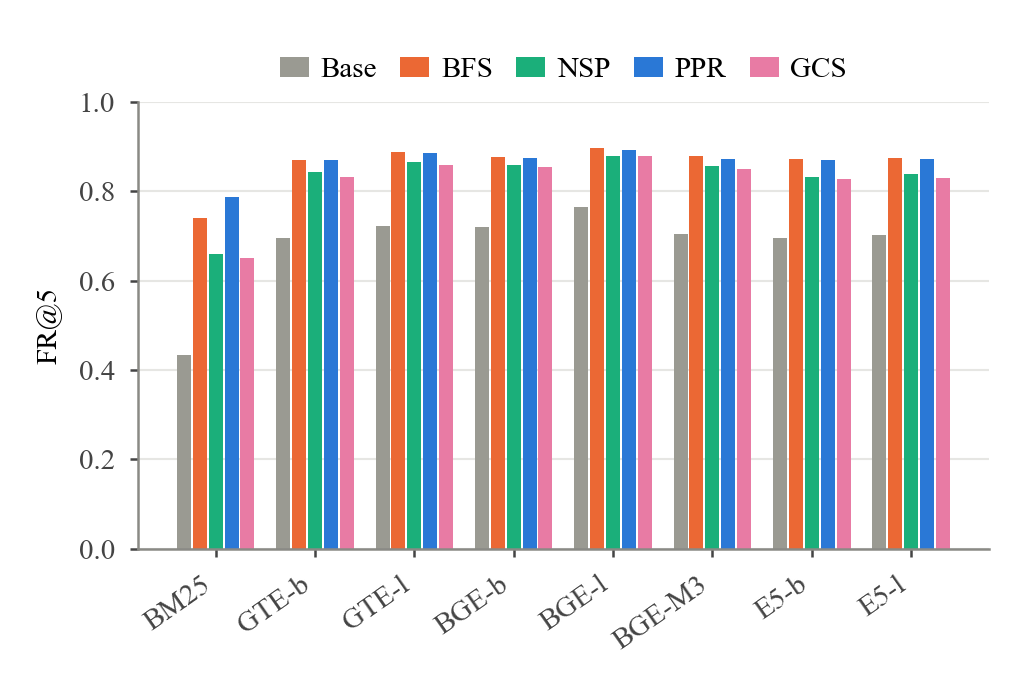
\includegraphics[width=\linewidth]{acl-style-files-master/img/Plot2Wiki.png}
    \caption{Wiki-based retrieval.}
    \label{fig:wiki_fr5}
\end{subfigure}
\hfill
\begin{subfigure}{0.31\textwidth}
    \centering
    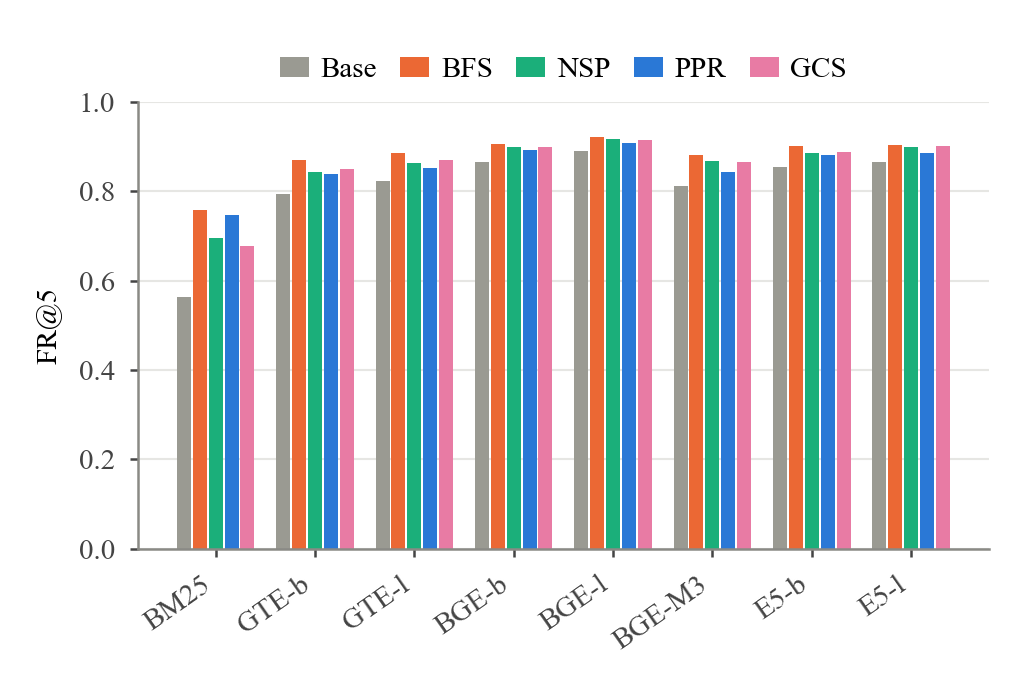
\includegraphics[width=\linewidth]{acl-style-files-master/img/PlotHotPot.png}
    \caption{HotpotQA dataset.}
    \label{fig:hotpot_fr5}
\end{subfigure}
\hfill
\begin{subfigure}{0.31\textwidth}
    \centering
    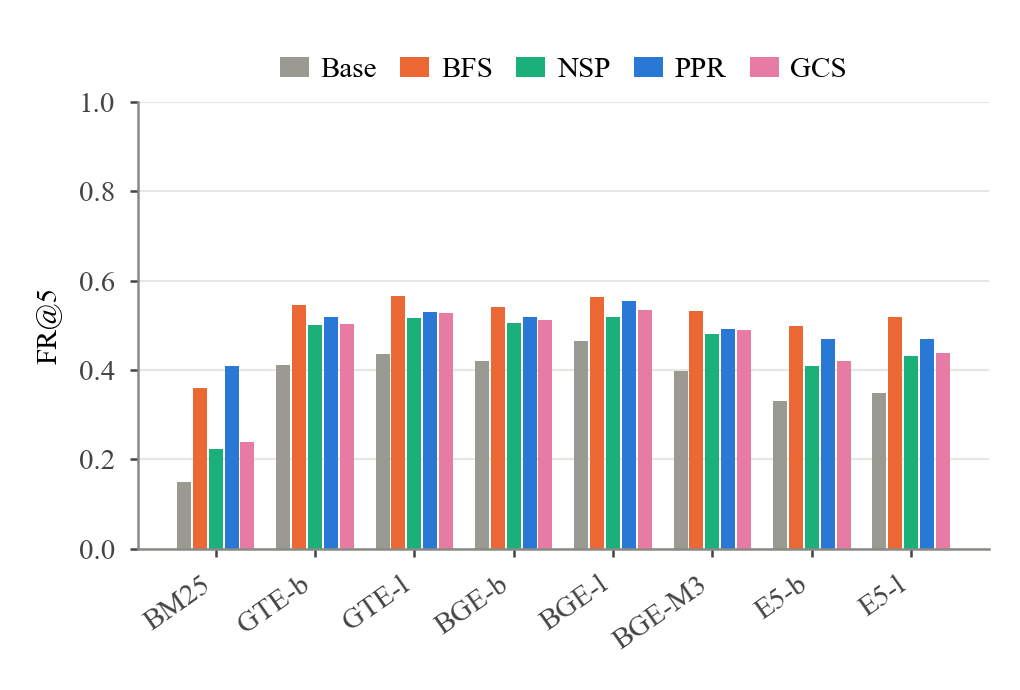
\includegraphics[width=\linewidth]{acl-style-files-master/img/PlotMusi.png}
    \caption{MuSiQue dataset.}
    \label{fig:musique_fr5}
\end{subfigure}

\caption{Full Recall (FR@5) comparison across datasets and retrieval models under Base, BFS, and NSP settings. Structured expansion methods consistently improve over the Base retriever, with BFS generally achieving the strongest performance across datasets.}
\label{fig:fr5_all}
\end{figure*}

\subsection{Ablation study}

The ablation study aims to observe the individual effects of entity and KG relation. We compare our main approach (utilizing both) to isolated graph construction strategies: entity-only, triple-only. 
Results show that integrating both entity-level overlaps and LLM-extracted semantic triples consistently yields the best retrieval performance. Entity-based edges strengthen dense local connectivity through repeated named entities, while triple-based edges provide precise semantic bridges that improve global reasoning and prevent graph expansion from becoming noisy or overly large.
Across retrieval methods, BFS performs best with shallow graph exploration (depth 1--2) and wider branching, as deeper traversal introduces irrelevant context. In contrast, graph embedding methods benefit from deeper propagation (2--3 hops), where the smoothing parameter $\alpha$ effectively controls information diffusion and maintains stable ranking quality without over-smoothing.


\section{Prediction analysis}

As can be seen from the results, the proposed method improves the performance of this class of models. At the same time, in the case of BFS, the BFS-based ranking process remains largely interpretable through graph traversal paths, and it is also possible to introduce a human-in-the-loop mechanism to correct samples when necessary. If we consider a sample from the MuSiQue dataset, the query is:

\begin{quote}
What was the director of The Accidental Husband nominated for?
\end{quote}

For this example, we consider a subsample of the retrieved passages (7 in total; the full text can be found in Appendix~\ref{appendix:list_text}). As shown in Table~\ref{tab:ranking_compact}, the model correctly ranks as relevant the passage with ID 6. However, the baseline struggles to retrieve other relevant passages. In the case of BFS, instead, three relevant passages improve their ranking, showing a better overall ordering. A similar behavior is observed with the NSP approach.

This behavior can be explained by the graph structure generated by the model, where nodes correspond to passage IDs and edges represent relationships between them. A key advantage of the BFS approach is its explainability: by selecting a top-$k$ value, it is possible to rerun the algorithm and inspect the reasoning behind each decision step. The graph constructed during the process is shown in Figure~\ref{fig:Graph}.

We observe that passages 0, 3, 6, 17, and 19 are strongly connected to each other, while passages 8 and 16 are relatively isolated. These isolated nodes are therefore treated as external and, as a consequence, tend to be ranked lower. In the BFS approach, passage 16 in particular receives a lower ranking due to its lack of connectivity, while passage 6 serves as a central node connecting multiple relevant passages.

In the NSP approach, the mechanism is different: if two elements are strongly related in the graph, their embeddings become similar. For this reason, passages 3 and 6 are closely related, which also contributes to improving the ranking of passage 3.

In contrast, in the BFS approach, the parameters are set such that $h = 3$ and the maximum exploration depth is 2 and the branch factor is 3. Therefore, the model first selects the three highest-ranked nodes, 6, 8 and 19. The node is isolated, so it is not expanded. Meanwhile 6 and 19 will explore near
From node 6, the expansion reaches nodes 19, 17, 3, and 0, which are then re-ranked based on similarity. Node 16, being isolated, remains at the bottom of the ranking. This makes the BFS approach for the higher positions more strict and bounded.


\begin{table}[t]
\centering
\footnotesize
\setlength{\tabcolsep}{3pt}
\renewcommand{\arraystretch}{0.85}
\begin{tabular}{lccccc}
\toprule
Method & 1 & 2 & 3 & 4 & 5 \\
\midrule
Base & 6$^\star$ & 8 & 19 & 16 & 3$^\star$ \\
BFS  & 6$^\star$ & 8 & 19 & 3$^\star$ & 17 \\
NSP  & 6$^\star$ & 8 & 3$^\star$ & 19 & 16 \\
\bottomrule
\end{tabular}
\caption{Ranking sequences, MuSiQue sample. $^\star$ = relevant.}
\label{tab:ranking_compact}
\end{table}





\begin{figure}[htb]
\centering
\includegraphics[scale=0.31]{acl-style-files-master/img/GrafoRetrivalEsempiPaper.png}
\caption{Textual Graph for MusiQue sample}
\label{fig:Graph}
\end{figure}
 




\section{Related Works}

Graph structures have been widely explored in information retrieval to model relationships between documents, entities, and contextual evidence, from early document-link and entity-based relevance propagation to recent graph-based RAG systems. GraphRAG~\cite{DBLP:conf/naacl/Hu2025} improves reasoning over large corpora via graph structure; T-GRAG~\cite{DBLP:journals/corr/Li2025TGRAG} adds temporal reasoning; TGLSTA~\cite{DBLP:conf/aaai/Zhang2025TGLSTA} combines semantic and structural graph learning with LLMs; and HippoRAG~\cite{DBLP:conf/nips/GutierrezS0Y024} uses entity and relation extraction to build structured representations for retrieval. In parallel, iterative multi-step retrieval~\cite{DBLP:conf/emnlp/SunBC19} expands context progressively but relies on query rewriting or sequential retrieval, adding complexity and instability.

Search+ differs from these methods mainly in \emph{when} and \emph{over what} the graph is built. HippoRAG constructs a persistent graph over the whole corpus at indexing time and retrieves via graph search directly; Search+ instead builds a lightweight, disposable graph only over the already-retrieved candidates, conditioned on the query, used solely as a post-hoc reranking layer on top of any existing retriever. Unlike HopRAG~\cite{DBLP:conf/acl/LiuWCLXYZ25}, which relies on iterative LLM reasoning during retrieval-time graph traversal, our approach performs a single graph construction pass per query using greedy decoding (temperature $=0$), followed by a deterministic traversal (e.g., BFS) and score propagation, yielding a fully reproducible pipeline without repeated LLM invocations during ranking.


\section{Limitations}

The proposed framework has limitations related to computational cost and reliance on LLMs, particularly for relational extraction during graph construction. While the graph-based ranking is lightweight, LLM inference introduces overhead and may inject prior knowledge that can bias results. We mitigate this by comparing against direct LLM reranking using the same model (Gemma 4 E4B), where our approach consistently performs better, as shown in Table~\ref{tab:llm_reranking}. We also observe that LLM-based reranking degrades as the number of passages increases, with issues such as unstable ranking outputs and occasional invalid JSON, especially on MuSiQue. In contrast, when used as a KG miner the model was more stable and less prone to hallucination.


\begin{table}[t]
\centering
\small
\begin{tabular}{lcc}
\toprule
\textbf{Dataset} & \textbf{Rank Direct LLM} & \textbf{Search+}\\
\midrule

2WikiMultiHopQA & 0.844 & 0.894\\
HotpotQA & 0.793 & 0.914 \\
MuSiQue & 0.311 & 0.557\\

\bottomrule
\end{tabular}
\caption{
Retrieval performance of direct LLM reranking vs our best method  reported using Full Recall@5.
}
\label{tab:llm_reranking}
\end{table}




\section{Conclusion and Future Work}\label{Conc}
In this work, we propose Search+, a graph-based framework for multi-hop information retrieval that organizes retrieved passages into a textual graph. Unlike standard retrieval methods that treat passages independently, our approach models relationships through shared entities and knowledge-based links.
We evaluate two strategies: Breadth-First Search (BFS) and Neighborhood Score Propagation (NSP). Experiments on HotpotQA, 2WikiMultiHopQA, and MuSiQue show consistent improvements across sparse and dense retrievers, with BFS achieving the strongest gains and improved interpretability.
The approach also serves as a higher-level ranking mechanism over top-k retrieved passages. Future work will explore reducing reliance on LLMs, integrating graph navigation strategies, improving entity matching, and learning better inter-passage relationships.




\section{Ethical Considerations and AI Assistance Disclosure}
In this work, we acknowledge the use of large language models for limited and non-substantive assistance, specifically for sentence-level reformulation, grammar correction, and debugging support in code implementation. These tools were not used for generating novel scientific claims, experimental design, or results interpretation.
All experiments were conducted using publicly available datasets (HotpotQA, 2WikiMultiHopQA, and MuSiQue), which do not contain sensitive, private, or personally identifiable information. Therefore, no ethical risks related to data privacy or human subjects are present in this study.
We emphasize that all methodological contributions, experimental setups, and scientific conclusions are the result of the authors' own work, with AI tools serving only as auxiliary writing and development aids.




\bibliography{custom}



\appendix

\section{Prompt for Textual Graph Construction}


\subsection{KG mining}
\label{appendix:KGM}
The following prompt was used to generate a textual graph representation from the input context. The model is instructed to extract only entities and relations relevant to the question and to output a structured JSON object.

\begin{quote}
\small
\texttt{You are a Knowledge Graph engineer.}

Given the question: \texttt{\{question\}}, analyze the following text: \texttt{\{context\}}.

\textbf{Task:} Extract the entities and relationships that are relevant for answering the question.

Return \textbf{ONLY} a valid JSON object containing:
\begin{itemize}
    \item \texttt{nodes}
    \item \texttt{edges}
\end{itemize}
\normalsize
\end{quote}


\subsection{Document Ranking LLM}

The following prompt was used to perform document ranking for information retrieval. The model is instructed to rank documents by relevance to the question and to output only a JSON list of document indices.

\begin{quote}
\small
\texttt{You are a document ranking system for information retrieval.}

\textbf{TASK:} \\
Rank documents by relevance to the question.

\textbf{STRICT OUTPUT RULES:}
\begin{itemize}
    \item ONLY output a JSON list of integers
    \item NO explanation
    \item NO extra text
\end{itemize}

\textbf{Example:} \\
\texttt{[2, 0, 1, 3]}

\textbf{QUESTION:} \\
\texttt{\{question\}}

\textbf{DOCUMENTS:} \\
\texttt{\{docs\}}
\normalsize
\end{quote}


\section{Full texts with ID}
\label{appendix:list_text}


It presents the list of all texts used in the sample MuSiQue.
\begin{table*}[t]
\centering
\begin{tabularx}{\textwidth}{c X}
\toprule
Node idx & Text \\
\midrule
0 & Geoffrey Drake (1911\u20131995) was an English production designer and art director. He was nominated for an Academy Award in the category Best Art Direction for the film \"Young Winston\".\\
3 & In 1995, Griffin Dunne was nominated for an Academy Award for Best Live Action Short Film for \"Duke of Groove\", which he directed and co-wrote. He shared the nomination with producer Thom Colwell. Along with his producing partner, actress/producer Amy Robinson, he has produced several films including \"Baby It's You\", \"After Hours\", \"Running on Empty\" and \"Game 6\" through their company, Double Play Productions.\\
6 & The Accidental Husband is a 2008 American romantic comedy film directed by Griffin Dunne, and starring Uma Thurman, Jeffrey Dean Morgan, Colin Firth, Isabella Rossellini, and Sam Shepard. The film was written by Mimi Hare, Clare Naylor and Bonnie Sikowitz, and is produced by Jennifer Todd, Jason Blum, and Uma Thurman. It was theatrically released in the UK in 2008, but was released direct-to-DVD in the United States.\\
8 & Open Water is a 2003 American survival horror - thriller film. The story concerns an American couple who go scuba diving while on vacation in the Caribbean, only to find themselves stranded miles from shore in shark - infested waters when the crew of their boat accidentally leaves them behind. The film is loosely based on the true story of Tom and Eileen Lonergan, who in 1998 went out with a scuba diving group, Outer Edge Dive Company, on the Great Barrier Reef, and were accidentally left behind because the dive - boat crew failed to take an accurate headcount. The film was financed by the husband and wife team of writer / director Chris Kentis and producer Laura Lau, both avid scuba divers. \\

16 & Tom Kuntz (born July 7, 1972) is an American director and filmmaker who is most known for his unique television commercials and music videos, which either have colorful settings, time-lapse photography or wildly eccentric humans. He has enjoyed multiple nominations for the honor of \u2018Best Commercial Director of the Year\u2019 by the DGA (Directors Guild of America; 2007, 2009, 2010, 2013, 2016)\\

17 & Gregory La Cava (March 10, 1892 \u2013 March 1, 1952) was an American film director of Italian descent best known for his films of the 1930s, including \"My Man Godfrey\" and \"Stage Door\", which earned him nominations for Academy Award for Best Director.\\

19 & Underground Secrets () is a 1991 Swedish drama film directed by Clas Lindberg. Lindberg won the award for Best Screenplay and was nominated for Best Director at the 27th Guldbagge Awards.\\

\bottomrule
\end{tabularx}
\caption{Evidence texts for all nodes.}
\label{tab:text_retrived}
\end{table*}

\newpage

\section{Complete results}


\label{appendix:all_results}

On the following three tables (Table \ref{tab:2wiki}, \ref{tab:Hot}, \ref{tab:Mu}), all the tests and ablation studies cited in the paper are presented. Each table corresponds to a single dataset test.

% % ==================== TABLE FOR DATASET: 2wiki_validation_test ====================
% ==================== TABLE FOR DATASET: 2wiki_validation_test ====================
\begin{table*}[t]
\centering
\footnotesize
\begin{tabular}{llllcccc}
\toprule
\textbf{Method} & \textbf{Mode} & \textbf{Type} & \textbf{Best Params} & \textbf{R@3} & \textbf{R@5} & \textbf{FR@3} & \textbf{FR@5} \\
\midrule

BM25 & Baseline & - & - & 0.6119 & 0.7270 & 0.2795 & 0.4320 \\
BM25 & BFS & triple & h: 3, d: 2, b: 3, $\alpha$: 1.0 & 0.6119 & 0.8617 & 0.2795 & 0.7077 \\
BM25 & BFS & entity & h: 3, d: 2, b: 5, $\alpha$: 1.0 & 0.6119 & 0.8596 & 0.2795 & 0.7027 \\
BM25 & BFS & both & h: 3, d: 2, b: 3, $\alpha$: 1.0 & 0.6119 & 0.8703 & 0.2795 & 0.7247 \\
BM25 & NSP & triple & hops: 3, $\alpha$: 0.3 & 0.6489 & 0.8062 & 0.3875 & 0.6152 \\
BM25 & NSP & entity & hops: 3, $\alpha$: 0.5 & 0.6477 & 0.8153 & 0.4025 & 0.6422 \\
BM25 & NSP & both & hops: 2, $\alpha$: 0.5 & 0.6625 & 0.8225 & 0.4250 & 0.6568 \\

GTE-base & Baseline & - & - & 0.7746 & 0.8702 & 0.5155 & 0.6925 \\
GTE-base & BFS & triple & h: 2, d: 3, b: 3, $\alpha$: 0.0 & 0.8393 & 0.9444 & 0.6105 & 0.8645 \\
GTE-base & BFS & entity & h: 2, d: 2, b: 10, $\alpha$: 0.0 & 0.8460 & 0.9405 & 0.6225 & 0.8545 \\
GTE-base & BFS & both & h: 2, d: 1, b: 10, $\alpha$: 1.0 & 0.8502 & 0.9414 & 0.6270 & 0.8595 \\
GTE-base & NSP & triple & hops: 3, $\alpha$: 0.2 & 0.8013 & 0.9114 & 0.5680 & 0.7920 \\
GTE-base & NSP & entity & hops: 3, $\alpha$: 0.5 & 0.8149 & 0.9297 & 0.6100 & 0.8420 \\
GTE-base & NSP & both & hops: 3, $\alpha$: 0.5 & 0.8103 & 0.9304 & 0.6060 & 0.8435 \\

GTE-large & Baseline & - & - & 0.7874 & 0.8838 & 0.5375 & 0.7215 \\
GTE-large & BFS & triple & h: 2, d: 2, b: 3, $\alpha$: 0.0 & 0.8478 & 0.9501 & 0.6230 & 0.8780 \\
GTE-large & BFS & entity & h: 2, d: 2, b: 3, $\alpha$: 1.0 & 0.8592 & 0.9501 & 0.6395 & 0.8795 \\
GTE-large & BFS & both & h: 2, d: 1, b: 5, $\alpha$: 1.0 & 0.8616 & 0.9517 & 0.6435 & 0.8815 \\
GTE-large & NSP & triple & hops: 3, $\alpha$: 0.3 & 0.8123 & 0.9221 & 0.5910 & 0.8200 \\
GTE-large & NSP & entity & hops: 3, $\alpha$: 0.5 & 0.8227 & 0.9400 & 0.6170 & 0.8635 \\
GTE-large & NSP & both & hops: 3, $\alpha$: 0.5 & 0.8215 & 0.9405 & 0.6205 & 0.8645 \\

BGE-base & Baseline & - & - & 0.7881 & 0.8826 & 0.5385 & 0.7195 \\
BGE-base & BFS & triple & h: 2, d: 3, b: 3, $\alpha$: 0.0 & 0.8459 & 0.9470 & 0.6230 & 0.8705 \\
BGE-base & BFS & entity & h: 2, d: 2, b: 10, $\alpha$: 0.0 & 0.8535 & 0.9464 & 0.6355 & 0.8680 \\
BGE-base & BFS & both & h: 2, d: 2, b: 5, $\alpha$: 0.0 & 0.8492 & 0.9463 & 0.6290 & 0.8700 \\
BGE-base & NSP & triple & hops: 3, $\alpha$: 0.2 & 0.8153 & 0.9221 & 0.5905 & 0.8160 \\
BGE-base & NSP & entity & hops: 3, $\alpha$: 0.3 & 0.8294 & 0.9371 & 0.6245 & 0.8540 \\
BGE-base & NSP & both & hops: 2, $\alpha$: 0.5 & 0.8269 & 0.9370 & 0.6250 & 0.8585 \\

BGE-large & Baseline & - & - & 0.8134 & 0.9064 & 0.5825 & 0.7640 \\
BGE-large & BFS & triple & h: 2, d: 2, b: 3, $\alpha$: 0.0 & 0.8601 & 0.9555 & 0.6460 & 0.8895 \\
BGE-large & BFS & entity & h: 2, d: 2, b: 3, $\alpha$: 0.0 & 0.8654 & 0.9546 & 0.6560 & 0.8900 \\
BGE-large & BFS & both & h: 2, d: 2, b: 5, $\alpha$: 0.0 & 0.8608 & 0.9567 & 0.6485 & 0.8940 \\
BGE-large & NSP & triple & hops: 3, $\alpha$: 0.2 & 0.8313 & 0.9365 & 0.6160 & 0.8440 \\
BGE-large & NSP & entity & hops: 1, $\alpha$: 0.5 & 0.8380 & 0.9475 & 0.6425 & 0.8775 \\
BGE-large & NSP & both & hops: 3, $\alpha$: 0.3 & 0.8401 & 0.9486 & 0.6425 & 0.8785 \\

BGE-M3 & Baseline & - & - & 0.7874 & 0.8742 & 0.5380 & 0.7035 \\
BGE-M3 & BFS & triple & h: 2, d: 2, b: 3, $\alpha$: 1.0 & 0.8584 & 0.9447 & 0.6405 & 0.8680 \\
BGE-M3 & BFS & entity & h: 3, d: 1, b: 3, $\alpha$: 1.0 & 0.7874 & 0.9416 & 0.5380 & 0.8585 \\
BGE-M3 & BFS & both & h: 2, d: 2, b: 3, $\alpha$: 1.0 & 0.8624 & 0.9463 & 0.6475 & 0.8715 \\
BGE-M3 & NSP & triple & hops: 3, $\alpha$: 0.3 & 0.8099 & 0.9205 & 0.5885 & 0.8160 \\
BGE-M3 & NSP & entity & hops: 3, $\alpha$: 0.5 & 0.8253 & 0.9326 & 0.6265 & 0.8460 \\
BGE-M3 & NSP & both & hops: 3, $\alpha$: 0.5 & 0.8207 & 0.9370 & 0.6225 & 0.8565 \\

E5-base & Baseline & - & - & 0.7775 & 0.8712 & 0.5340 & 0.6945 \\
E5-base & BFS & triple & h: 2, d: 3, b: 3, $\alpha$: 0.0 & 0.8419 & 0.9435 & 0.6210 & 0.8645 \\
E5-base & BFS & entity & h: 2, d: 2, b: 5, $\alpha$: 0.0 & 0.8464 & 0.9436 & 0.6265 & 0.8640 \\
E5-base & BFS & both & h: 2, d: 1, b: 10, $\alpha$: 1.0 & 0.8549 & 0.9444 & 0.6415 & 0.8665 \\
E5-base & NSP & triple & hops: 2, $\alpha$: 0.3 & 0.8005 & 0.9091 & 0.5860 & 0.7875 \\
E5-base & NSP & entity & hops: 2, $\alpha$: 0.5 & 0.8087 & 0.9245 & 0.6120 & 0.8285 \\
E5-base & NSP & both & hops: 2, $\alpha$: 0.5 & 0.8074 & 0.9253 & 0.6130 & 0.8315 \\

E5-large & Baseline & - & - & 0.7741 & 0.8702 & 0.5295 & 0.7010 \\
E5-large & BFS & triple & h: 2, d: 3, b: 3, $\alpha$: 0.0 & 0.8397 & 0.9445 & 0.6175 & 0.8655 \\
E5-large & BFS & entity & h: 2, d: 2, b: 3, $\alpha$: 1.0 & 0.8519 & 0.9417 & 0.6340 & 0.8640 \\
E5-large & BFS & both & h: 2, d: 2, b: 10, $\alpha$: 1.0 & 0.8512 & 0.9425 & 0.6310 & 0.8635 \\
E5-large & NSP & triple & hops: 2, $\alpha$: 0.3 & 0.8027 & 0.9100 & 0.5890 & 0.7960 \\
E5-large & NSP & entity & hops: 3, $\alpha$: 0.5 & 0.8075 & 0.9269 & 0.6105 & 0.8370 \\
E5-large & NSP & both & hops: 2, $\alpha$: 0.5 & 0.8065 & 0.9269 & 0.6115 & 0.8385 \\

\bottomrule
\end{tabular}
\caption{2Wiki validation test (normalized parameters).}
\label{tab:2wiki}
\end{table*}
% ==================== TABLE FOR DATASET: hotpotqa_validation_test ====================
\begin{table*}[t]
\centering
\footnotesize
\begin{tabular}{llllcccc}
\toprule
\textbf{Method} & \textbf{Mode} & \textbf{Type} & \textbf{Best Params} & \textbf{R@3} & \textbf{R@5} & \textbf{FR@3} & \textbf{FR@5} \\
\midrule

BM25 & Baseline & - & - & 0.6515 & 0.7663 & 0.3775 & 0.5630 \\
BM25 & BFS & triple & h: 3, d: 2, b: 3, $\alpha$: 1.0 & 0.6515 & 0.8622 & 0.3775 & 0.7445 \\
BM25 & BFS & entity & h: 3, d: 2, b: 5, $\alpha$: 1.0 & 0.6515 & 0.8395 & 0.3775 & 0.7045 \\
BM25 & BFS & both & h: 3, d: 2, b: 3, $\alpha$: 1.0 & 0.6515 & 0.8630 & 0.3775 & 0.7450 \\
BM25 & NSP & triple & hops: 3, $\alpha$: 0.2 & 0.6555 & 0.7938 & 0.4050 & 0.6235 \\
BM25 & NSP & entity & hops: 3, $\alpha$: 0.5 & 0.6713 & 0.8128 & 0.4695 & 0.6835 \\
BM25 & NSP & both & hops: 3, $\alpha$: 0.5 & 0.6762 & 0.8180 & 0.4770 & 0.6920 \\

GTE-base & Baseline & - & - & 0.8067 & 0.8902 & 0.6400 & 0.7920 \\
GTE-base & BFS & triple & h: 2, d: 3, b: 3, $\alpha$: 0.0 & 0.8438 & 0.9280 & 0.7075 & 0.8645 \\
GTE-base & BFS & entity & h: 3, d: 2, b: 5, $\alpha$: 0.0 & 0.8067 & 0.9173 & 0.6400 & 0.8460 \\
GTE-base & BFS & both & h: 3, d: 2, b: 3, $\alpha$: 1.0 & 0.8067 & 0.9263 & 0.6400 & 0.8610 \\
GTE-base & NSP & triple & hops: 2, $\alpha$: 0.2 & 0.8033 & 0.8985 & 0.6410 & 0.8090 \\
GTE-base & NSP & entity & hops: 2, $\alpha$: 0.3 & 0.8277 & 0.9135 & 0.6900 & 0.8430 \\
GTE-base & NSP & both & hops: 2, $\alpha$: 0.3 & 0.8260 & 0.9127 & 0.6860 & 0.8410 \\

GTE-large & Baseline & - & - & 0.8293 & 0.9062 & 0.6845 & 0.8220 \\
GTE-large & BFS & triple & h: 2, d: 2, b: 3, $\alpha$: 0.0 & 0.8608 & 0.9343 & 0.7375 & 0.8755 \\
GTE-large & BFS & entity & h: 3, d: 1, b: 10, $\alpha$: 0.0 & 0.8293 & 0.9270 & 0.6845 & 0.8630 \\
GTE-large & BFS & both & h: 3, d: 1, b: 3, $\alpha$: 1.0 & 0.8293 & 0.9347 & 0.6845 & 0.8755 \\
GTE-large & NSP & triple & hops: 3, $\alpha$: 0.2 & 0.8087 & 0.9073 & 0.6555 & 0.8250 \\
GTE-large & NSP & entity & hops: 2, $\alpha$: 0.3 & 0.8490 & 0.9243 & 0.7315 & 0.8600 \\
GTE-large & NSP & both & hops: 2, $\alpha$: 0.3 & 0.8423 & 0.9255 & 0.7175 & 0.8630 \\

BGE-base & Baseline & - & - & 0.8620 & 0.9295 & 0.7395 & 0.8645 \\
BGE-base & BFS & triple & h: 2, d: 1, b: 3, $\alpha$: 0.0 & 0.8852 & 0.9487 & 0.7805 & 0.9010 \\
BGE-base & BFS & entity & h: 3, d: 2, b: 5, $\alpha$: 0.0 & 0.8620 & 0.9417 & 0.7395 & 0.8890 \\
BGE-base & BFS & both & h: 3, d: 1, b: 5, $\alpha$: 0.0 & 0.8620 & 0.9440 & 0.7395 & 0.8930 \\
BGE-base & NSP & triple & hops: 3, $\alpha$: 0.1 & 0.8600 & 0.9333 & 0.7385 & 0.8720 \\
BGE-base & NSP & entity & hops: 3, $\alpha$: 0.2 & 0.8770 & 0.9467 & 0.7720 & 0.9010 \\
BGE-base & NSP & both & hops: 3, $\alpha$: 0.2 & 0.8738 & 0.9460 & 0.7670 & 0.8995 \\

BGE-large & Baseline & - & - & 0.8902 & 0.9435 & 0.7895 & 0.8905 \\
BGE-large & BFS & triple & h: 2, d: 1, b: 3, $\alpha$: 0.0 & 0.9070 & 0.9585 & 0.8215 & 0.9195 \\
BGE-large & BFS & entity & h: 1, d: 1, b: 5, $\alpha$: 0.0 & 0.8612 & 0.9535 & 0.7340 & 0.9105 \\
BGE-large & BFS & both & h: 3, d: 1, b: 5, $\alpha$: 0.0 & 0.8902 & 0.9553 & 0.7895 & 0.9140 \\
BGE-large & NSP & triple & hops: 3, $\alpha$: 0.1 & 0.8870 & 0.9475 & 0.7850 & 0.8985 \\
BGE-large & NSP & entity & hops: 2, $\alpha$: 0.3 & 0.9022 & 0.9575 & 0.8170 & 0.9185 \\
BGE-large & NSP & both & hops: 2, $\alpha$: 0.3 & 0.9005 & 0.9567 & 0.8120 & 0.9170 \\

E5-base & Baseline & - & - & 0.8472 & 0.9235 & 0.7165 & 0.8545 \\
E5-base & BFS & triple & h: 3, d: 1, b: 3, $\alpha$: 0.5 & 0.8472 & 0.9503 & 0.7165 & 0.9045 \\
E5-base & BFS & entity & h: 1, d: 1, b: 3, $\alpha$: 0.3 & 0.8277 & 0.9410 & 0.6795 & 0.8895 \\
E5-base & BFS & both & h: 1, d: 1, b: 3, $\alpha$: 0.3 & 0.8452 & 0.9487 & 0.7070 & 0.9020 \\
E5-base & NSP & triple & hops: 3, $\alpha$: 0.2 & 0.8337 & 0.9245 & 0.6990 & 0.8565 \\
E5-base & NSP & entity & hops: 2, $\alpha$: 0.3 & 0.8665 & 0.9390 & 0.7595 & 0.8880 \\
E5-base & NSP & both & hops: 1, $\alpha$: 0.5 & 0.8582 & 0.9377 & 0.7475 & 0.8855 \\

E5-large & Baseline & - & - & 0.8582 & 0.9310 & 0.7305 & 0.8660 \\
E5-large & BFS & triple & h: 3, d: 2, b: 3, $\alpha$: 0.3 & 0.8582 & 0.9527 & 0.7305 & 0.9075 \\
E5-large & BFS & entity & h: 1, d: 1, b: 3, $\alpha$: 0.3 & 0.8405 & 0.9467 & 0.6970 & 0.8980 \\
E5-large & BFS & both & h: 1, d: 1, b: 3, $\alpha$: 0.7 & 0.8450 & 0.9507 & 0.7005 & 0.9035 \\
E5-large & NSP & triple & hops: 3, $\alpha$: 0.1 & 0.8628 & 0.9380 & 0.7430 & 0.8805 \\
E5-large & NSP & entity & hops: 2, $\alpha$: 0.3 & 0.8780 & 0.9470 & 0.7750 & 0.8985 \\
E5-large & NSP & both & hops: 2, $\alpha$: 0.3 & 0.8780 & 0.9470 & 0.7750 & 0.8985 \\

\bottomrule
\end{tabular}
\caption{HotpotQA validation test (normalized parameters).}
\label{tab:Hot}
\end{table*}


% ==================== TABLE FOR DATASET: musique_validation_test ====================
\begin{table*}[t]
\centering
\footnotesize
\begin{tabular}{llllcccc}
\toprule
\textbf{Method} & \textbf{Mode} & \textbf{Type} & \textbf{Best Params} & \textbf{R@3} & \textbf{R@5} & \textbf{FR@3} & \textbf{FR@5} \\
\midrule

BM25 & Baseline & - & - & 0.3846 & 0.4930 & 0.0711 & 0.1472 \\
BM25 & BFS & triple & h: 3, d: 2, b: 3, $\alpha$: 1.0 & 0.3846 & 0.6212 & 0.0711 & 0.3499 \\
BM25 & BFS & entity & h: 3, d: 2, b: 3, $\alpha$: 0.0 & 0.3846 & 0.5939 & 0.0711 & 0.3176 \\
BM25 & BFS & both & h: 3, d: 2, b: 3, $\alpha$: 1.0 & 0.3846 & 0.6228 & 0.0711 & 0.3548 \\
BM25 & NSP & triple & hops: 2, $\alpha$: 0.2 & 0.3747 & 0.4979 & 0.1009 & 0.1902 \\
BM25 & NSP & entity & hops: 1, $\alpha$: 0.5 & 0.3697 & 0.5037 & 0.1224 & 0.2275 \\
BM25 & NSP & both & hops: 1, $\alpha$: 0.5 & 0.3656 & 0.5012 & 0.1216 & 0.2225 \\

GTE-base & Baseline & - & - & 0.5962 & 0.7135 & 0.2473 & 0.4111 \\
GTE-base & BFS & triple & h: 1, d: 3, b: 3, $\alpha$: 0.0 & 0.6561 & 0.7748 & 0.3540 & 0.5451 \\
GTE-base & BFS & entity & h: 3, d: 2, b: 5, $\alpha$: 0.0 & 0.5962 & 0.7727 & 0.2473 & 0.5244 \\
GTE-base & BFS & both & h: 3, d: 1, b: 3, $\alpha$: 1.0 & 0.5962 & 0.7716 & 0.2473 & 0.5318 \\
GTE-base & NSP & triple & hops: 1, $\alpha$: 0.3 & 0.6062 & 0.7333 & 0.2812 & 0.4624 \\
GTE-base & NSP & entity & hops: 1, $\alpha$: 0.5 & 0.6132 & 0.7541 & 0.3151 & 0.5045 \\
GTE-base & NSP & both & hops: 1, $\alpha$: 0.5 & 0.6124 & 0.7493 & 0.3102 & 0.5012 \\

GTE-large & Baseline & - & - & 0.6114 & 0.7290 & 0.2622 & 0.4334 \\
GTE-large & BFS & triple & h: 1, d: 2, b: 3, $\alpha$: 0.0 & 0.6669 & 0.7847 & 0.3581 & 0.5476 \\
GTE-large & BFS & entity & h: 3, d: 2, b: 5, $\alpha$: 0.0 & 0.6114 & 0.7838 & 0.2622 & 0.5426 \\
GTE-large & BFS & both & h: 3, d: 2, b: 3, $\alpha$: 0.0 & 0.6114 & 0.7846 & 0.2622 & 0.5467 \\
GTE-large & NSP & triple & hops: 3, $\alpha$: 0.2 & 0.6164 & 0.7517 & 0.3019 & 0.4905 \\
GTE-large & NSP & entity & hops: 1, $\alpha$: 0.5 & 0.6365 & 0.7652 & 0.3391 & 0.5261 \\
GTE-large & NSP & both & hops: 1, $\alpha$: 0.5 & 0.6273 & 0.7630 & 0.3284 & 0.5161 \\

BGE-base & Baseline & - & - & 0.5895 & 0.7089 & 0.2473 & 0.4194 \\
BGE-base & BFS & triple & h: 3, d: 2, b: 3, $\alpha$: 1.0 & 0.5895 & 0.7670 & 0.2473 & 0.5302 \\
BGE-base & BFS & entity & h: 2, d: 3, b: 5, $\alpha$: 0.0 & 0.6505 & 0.7571 & 0.3639 & 0.5219 \\
BGE-base & BFS & both & h: 3, d: 2, b: 3, $\alpha$: 1.0 & 0.5895 & 0.7594 & 0.2473 & 0.5203 \\
BGE-base & NSP & triple & hops: 3, $\alpha$: 0.2 & 0.5919 & 0.7263 & 0.2771 & 0.4739 \\
BGE-base & NSP & entity & hops: 3, $\alpha$: 0.3 & 0.6101 & 0.7352 & 0.3259 & 0.5029 \\
BGE-base & NSP & both & hops: 1, $\alpha$: 0.5 & 0.6103 & 0.7373 & 0.3242 & 0.5062 \\

BGE-large & Baseline & - & - & 0.6099 & 0.7461 & 0.2779 & 0.4648 \\
BGE-large & BFS & triple & h: 1, d: 3, b: 3, $\alpha$: 0.0 & 0.6624 & 0.7866 & 0.3730 & 0.5492 \\
BGE-large & BFS & entity & h: 2, d: 3, b: 3, $\alpha$: 0.0 & 0.6685 & 0.7863 & 0.3888 & 0.5575 \\
BGE-large & BFS & both & h: 2, d: 2, b: 5, $\alpha$: 0.0 & 0.6614 & 0.7867 & 0.3772 & 0.5575 \\
BGE-large & NSP & triple & hops: 3, $\alpha$: 0.1 & 0.6181 & 0.7537 & 0.3069 & 0.4880 \\
BGE-large & NSP & entity & hops: 2, $\alpha$: 0.3 & 0.6321 & 0.7665 & 0.3400 & 0.5269 \\
BGE-large & NSP & both & hops: 3, $\alpha$: 0.2 & 0.6256 & 0.7606 & 0.3259 & 0.5178 \\

BGE-M3 & Baseline & - & - & 0.5823 & 0.7070 & 0.2266 & 0.3987 \\
BGE-M3 & BFS & triple & h: 3, d: 2, b: 3, $\alpha$: 1.0 & 0.5823 & 0.7692 & 0.2266 & 0.5161 \\
BGE-M3 & BFS & entity & h: 3, d: 2, b: 5, $\alpha$: 0.0 & 0.5823 & 0.7656 & 0.2266 & 0.5128 \\
BGE-M3 & BFS & both & h: 3, d: 2, b: 3, $\alpha$: 1.0 & 0.5823 & 0.7663 & 0.2266 & 0.5136 \\
BGE-M3 & NSP & triple & hops: 3, $\alpha$: 0.2 & 0.5948 & 0.7283 & 0.2878 & 0.4615 \\
BGE-M3 & NSP & entity & hops: 2, $\alpha$: 0.5 & 0.5951 & 0.7368 & 0.3251 & 0.4946 \\
BGE-M3 & NSP & both & hops: 1, $\alpha$: 0.5 & 0.6032 & 0.7333 & 0.3184 & 0.4814 \\

E5-base & Baseline & - & - & 0.5332 & 0.6485 & 0.2026 & 0.3309 \\
E5-base & BFS & triple & h: 3, d: 2, b: 5, $\alpha$: 1.0 & 0.5332 & 0.7228 & 0.2026 & 0.4640 \\
E5-base & BFS & entity & h: 2, d: 3, b: 5, $\alpha$: 0.0 & 0.6002 & 0.7195 & 0.3226 & 0.4773 \\
E5-base & BFS & both & h: 3, d: 2, b: 10, $\alpha$: 1.0 & 0.5332 & 0.7232 & 0.2026 & 0.4715 \\
E5-base & NSP & triple & hops: 2, $\alpha$: 0.2 & 0.5403 & 0.6676 & 0.2390 & 0.3797 \\
E5-base & NSP & entity & hops: 1, $\alpha$: 0.5 & 0.5505 & 0.6817 & 0.2804 & 0.4194 \\
E5-base & NSP & both & hops: 1, $\alpha$: 0.5 & 0.5372 & 0.6744 & 0.2655 & 0.4078 \\

E5-large & Baseline & - & - & 0.5399 & 0.6548 & 0.2159 & 0.3490 \\
E5-large & BFS & triple & h: 2, d: 3, b: 3, $\alpha$: 0.0 & 0.6148 & 0.7370 & 0.3292 & 0.4955 \\
E5-large & BFS & entity & h: 2, d: 3, b: 5, $\alpha$: 0.0 & 0.6137 & 0.7288 & 0.3383 & 0.4880 \\
E5-large & BFS & both & h: 3, d: 2, b: 10, $\alpha$: 1.0 & 0.5399 & 0.7313 & 0.2159 & 0.4897 \\
E5-large & NSP & triple & hops: 3, $\alpha$: 0.3 & 0.5562 & 0.6737 & 0.2589 & 0.3925 \\
E5-large & NSP & entity & hops: 3, $\alpha$: 0.3 & 0.5653 & 0.6948 & 0.2808 & 0.4289 \\
E5-large & NSP & both & hops: 3, $\alpha$: 0.3 & 0.5542 & 0.6873 & 0.2833 & 0.4355 \\

\bottomrule
\end{tabular}
\caption{MuSiQue validation test (fully expanded, normalized parameters).}
\label{tab:Mu}

\end{table*}

\newpage


\end{document}